\documentclass[xcolor=table]{beamer}
%------------------------------------------------------------
% Theme and Appearance
%------------------------------------------------------------
\usetheme[footline=authorinstitutetitle]{Berlin} 
\setbeamertemplate{navigation symbols}{} 

% Headline with Access Code
\setbeamertemplate{headline}{
    \begin{beamercolorbox}[wd=\paperwidth,ht=2.5ex,dp=1ex,right]{section in head/foot}
        \usebeamerfont{section in head/foot}
        \hspace{0.5cm}
        \ifnum\insertframenumber<30
            \raisebox{-1pt}[0pt][0pt]{\normalsize\textbf{Attendance Code: 123456}}
        \fi
        \hspace{0.5cm}
    \end{beamercolorbox}
}
% Footline with page numbers
\setbeamertemplate{footline}{
    \leavevmode%
    \hbox{%
        \begin{beamercolorbox}[wd=.333333\paperwidth,ht=2.25ex,dp=1ex,left]{author in head/foot}%
            \usebeamerfont{author in head/foot}\hspace*{0.5em}\insertshortauthor
        \end{beamercolorbox}%
        \begin{beamercolorbox}[wd=.333333\paperwidth,ht=2.25ex,dp=1ex,center]{title in head/foot}%
            \usebeamerfont{title in head/foot}\insertshorttitle
        \end{beamercolorbox}%
        \begin{beamercolorbox}[wd=.333333\paperwidth,ht=2.25ex,dp=1ex,right]{date in head/foot}%
            \usebeamerfont{date in head/foot}\insertshortdate{}\hspace*{2em}
            \insertframenumber{} / \inserttotalframenumber\hspace*{2ex} 
        \end{beamercolorbox}}%
    \vskip0pt%
}
\usepackage[utf8]{inputenc}
\usepackage[table]{xcolor}
\usepackage{colortbl}
\usepackage{minted}
\usepackage{lmodern}
\usepackage{tgheros}
\usepackage{hyperref}
\usepackage{tikz}
\usetikzlibrary{shapes, arrows, arrows.meta, positioning, shadows, fit, calc, backgrounds, decorations.pathreplacing}

\renewcommand*\familydefault{\sfdefault}

% Agenda at the start of every section
\AtBeginSection[]
{
    \begin{frame}
        \frametitle{Agenda}
        \tableofcontents[currentsection]
    \end{frame}
}

%------------------------------------------------------------
% Title Page Information
%------------------------------------------------------------
\title[CMP9134 - Week 14]{Legal, Ethical, Professional, and Social Issues in Software Engineering}
\subtitle{CMP9134: Software Engineering}
\author[Francesco Del Duchetto]{Dr Francesco Del Duchetto\\Lecturer in Robotics and Autonomous Systems}
\institute[University of Lincoln]{University of Lincoln}
\date{08 May 2026}

%------------------------------------------------------------
\begin{document}

%--- TITLE FRAME ---
\begin{frame}
    \titlepage
\end{frame}

%--- AGENDA FRAME ---
\begin{frame}
    \frametitle{Today's Agenda}
    \tableofcontents
\end{frame}

%------------------------------------------------------------
\section{The Professional Engineer}
%------------------------------------------------------------

\begin{frame}
    \frametitle{Revisiting LEPSI}
    In Week 3, we introduced \textbf{LEPSI} (Legal, Ethical, Professional, and Social Issues) as strict Non-Functional Requirements (NFRs).
    
    \vspace{0.3cm}
    You learned that things like GDPR, CCPA, and HIPAA dictate how you design your databases. You also learned about WCAG accessibility standards.
    
    \vspace{0.3cm}
    Today, we move beyond basic compliance. We will explore the complex ethical realities of modern software engineering, intellectual property, and provide a structured framework for writing academic reflections on your engineering decisions.
\end{frame}

\begin{frame}
    \frametitle{The Professional Code of Conduct}
    \small
    Software Engineering is a recognized profession. Like doctors or civil engineers, we are bound by Codes of Conduct, such as the ACM/IEEE-CS Code of Ethics.
    
    \vspace{0.2cm}
    \begin{block}{ACM Code of Ethics \& Professional Practice}
        Key principles include:
        \begin{itemize}
            \item \textbf{Public:} Software engineers shall act consistently with the public interest.
            \item \textbf{Product:} Ensure that products meet the highest professional standards possible.
            \item \textbf{Judgment:} Maintain integrity and independence in professional judgment.
            \item \textbf{Colleagues:} Be fair to and supportive of colleagues.
        \end{itemize}
    \end{block}
\end{frame}

\begin{frame}
    % \being{center}
    
\includegraphics[width=1\textwidth]{CoC.png}
    % \end{center}

    \url{https://www.acm.org/code-of-ethics/software-engineering-code}
\end{frame}

\begin{frame}
    \frametitle{When Professionalism Fails: Volkswagen}
    \small
    What happens when technical constraints override ethical judgment?
    
    \vspace{0.2cm}
    \textbf{The Volkswagen Emissions Scandal (2015)}
    \begin{itemize}
        \item Volkswagen intentionally programmed diesel engine vehicles to activate emission controls \textit{only} during laboratory testing.
        \item On the road, vehicles output more than 40 times the allowed NOx limits.
        \item \textbf{Why?} Engineers were unable to meet EPA requirements in the allotted time and budget. Faced with a toxic work culture, they opted to rig the software test rather than fix the engineering problem.
        \item \textbf{Result:} It cost the company over 31 billion euros and led to arrests of top executives.
    \end{itemize}
\end{frame}

%------------------------------------------------------------
\section{Intellectual Property \& Licensing}
%------------------------------------------------------------

\begin{frame}
    \frametitle{Intellectual Property (IP) in Software}
    \small
    Intellectual property refers to creations of the mind. IP rights are crucial to protecting software and code.
    
    \vspace{0.2cm}
    \begin{itemize}
        \item \textbf{Copyrights:} Protect original works of authorship, such as artwork, software code and documentation.
        \item \textbf{Patents:} Protect inventions, such as new software algorithms or processes.
        \item \textbf{Trademarks:} Protect symbols, names, and logos.
        \item \textbf{Trade Secrets:} Protect confidential information, such as proprietary algorithms. These do not expire as long as they remain secret.
    \end{itemize}
\end{frame}

\begin{frame}
    \frametitle{Copyright}
    \small
    \begin{itemize}
        \item Copyright protects original work of authorship, including code and documentation.
        \item It grants the creator exclusive rights to reproduce, distribute, and create derivative works.
        \item In software, copyright is automatically granted when you write code. It does not protect ideas, only the expression of those ideas (e.g., the specific code you write, not the underlying algorithm).
    \end{itemize}
\end{frame}

\begin{frame}
    \frametitle{Software Licensing Models}
    \small
    License compliance is critical to ensure software is used legally.
    
    \vspace{0.2cm}
    \textbf{1. Proprietary Licensing:} Software owned by a specific company with strict restrictions on use and modification (e.g., Microsoft 365, Adobe).
    
    \vspace{0.2cm}
    \textbf{2. Open Source Licensing:} Distributed under a license that allows users to access, modify, and distribute the source code.
    \begin{itemize}
        \item \textbf{Permissive (e.g., MIT, Apache):} Allows users to modify and distribute software under highly flexible terms without requiring derivatives to share the same license.
        \item \textbf{Copyleft (e.g., GNU GPL):} Requires any modifications or derivatives of the software to be distributed under the \textit{exact same license}.
    \end{itemize}

    Help for choosing the right license: \url{https://choosealicense.com/}
\end{frame}

\begin{frame}
    \frametitle{Knowledge Check:}
    \textbf{Scenario:} 
    You build a proprietary, closed-source web dashboard for a commercial client. 
    
    To save time, you import a highly advanced data-visualisation library from GitHub. You check the license, and it is licensed under \textbf{GPLv3} (Copyleft).
    
    \vspace{0.3cm}
    \textbf{Question:} What is the legal implication of this engineering decision?
    
    \pause
    \vspace{0.2cm}
    \begin{alertblock}{Answer}
        Copyleft licenses ensure software remains open source. By linking a GPL library into your proprietary app and distributing it, your entire dashboard legally becomes subject to the GPL. You must publish all your proprietary source code for free!
    \end{alertblock}
\end{frame}

\begin{frame}
    \frametitle{Patents}
    \small
    Patents protect inventions, such as new software algorithms or processes. They grant the patent holder exclusive rights to use and commercialize the invention for a limited time (usually 20 years).

    \vspace{0.2cm}
    \textbf{Examples of Software Patents:}
    \begin{itemize}
        \item Google's PageRank algorithm (used in search engines).
        \item Amazon's 1-Click ordering system (used in e-commerce).
        \item Apple's slide-to-unlock feature (used in mobile devices).
    \end{itemize}
\end{frame}

\begin{frame}
    \frametitle{Trademarks \& Trade Secrets}
    \small
    \textbf{Trademarks} protect symbols, names, and logos that distinguish products or services (e.g., the Windows logo, the Apple logo).
    
    \vspace{0.2cm}
    \textbf{Trade Secrets} protect confidential information that provides a competitive edge. They do not expire as long as they remain secret (e.g., Google's exact search algorithm). These are protected through non-disclosure agreements (NDAs) and internal security measures.
    
    \vspace{0.2cm}
    Both are crucial for brand identity and competitive advantage in the software industry.

\end{frame}

\begin{frame}
    \frametitle{IP Infringement \& Consequences}
    \small
    IP infringement occurs when someone uses, reproduces, or distributes protected intellectual property without permission. This can include copying code, using patented algorithms, or misusing trademarks.

    \vspace{0.2cm}
    Infringing on intellectual property can lead to severe legal consequences, including:
    \begin{itemize}
        \item \textbf{Lawsuits:} IP holders can sue for damages, which can result in costly settlements or judgments.
        \item \textbf{Injunctions:} Courts can order the infringing party to stop using the IP, which can disrupt business operations.
    \end{itemize}

\end{frame}

%------------------------------------------------------------
\section{Security \& Ethical Hacking}
%------------------------------------------------------------

\begin{frame}
    \frametitle{Cybersecurity \& Ethical Hacking}
    \small
    Cybersecurity ensures that software is secure and protects against cyber threats through secure coding, testing, and encryption.
    
    \vspace{0.2cm}
    \textbf{Ethical Hacking} is testing systems to identify vulnerabilities before malicious actors can exploit them. It must be conducted legally and respectfully.
    
    \begin{itemize}
        \item \textbf{Process:} Planning/scoping $\rightarrow$ Reconnaissance $\rightarrow$ Vulnerability scanning $\rightarrow$ Exploitation $\rightarrow$ Reporting.
        \item \textbf{Types:} Network penetration testing, web application testing, and Social Engineering (e.g., phishing emails to test employee awareness).
        \item \textbf{Hacktivism:} Using hacking as civil disobedience to promote human rights or freedom of information (e.g., WikiLeaks).
    \end{itemize}
\end{frame}

%------------------------------------------------------------
\section{Decolonisation \& AI Ethics}
%------------------------------------------------------------

\begin{frame}
    \frametitle{What is (not) Decolonisation?}
    \footnotesize
    \begin{block}{Decolonisation is...}
        \begin{itemize}
            \item A \textbf{critical process} of questioning who defines "good" technology and whose knowledge is treated as valid.
            \item Redistributing power: involving local communities, languages, and lived realities in decisions.
            \item Changing systems (data pipelines, standards, governance), not just changing wording.
        \end{itemize}
    \end{block}

    % \vspace{0.2cm}
    \begin{alertblock}{Decolonisation is \textit{not}...}
        \begin{itemize}
            \item A metaphor for generic improvement, innovation, or adding "diversity" as a checkbox.
            \item A one-off workshop, statement, or rebrand with no change in ownership or accountability.
            \item Rejecting all Western knowledge; it is about plurality, context, and equitable participation.
        \end{itemize}
    \end{alertblock}
\end{frame}


\begin{frame}
    \frametitle{What is Decolonisation in Tech?}
    Historically, colonisation was about physical borders and resource extraction. Modern decolonisation in academia and tech addresses \textbf{Epistemic Borders} (whose knowledge, data, and culture are prioritized).
    
    \vspace{0.3cm}
    \begin{block}{Data Colonialism (Couldry \& Mejias, 2018)}
        The appropriation of human life through data extraction. Western tech giants extract data globally, process it centrally, and sell algorithms back to the world, often enforcing singular cultural norms on diverse populations. \url{https://doi.org/10.1177/1527476418796632}
    \end{block}
\end{frame}

\begin{frame}
    \frametitle{Case Study: Surveillance Tech in Palestine}
    \footnotesize
    This case is often discussed in decolonisation debates as an example of how digital systems can be developed and refined under conditions of occupation.

    \vspace{0.2cm}
    \begin{itemize}
        \item Human rights reports document extensive biometric and predictive surveillance infrastructures used on Palestinians in the occupied Palestinian territory.
        \item Reported systems include facial recognition at checkpoints and large-scale data integration for movement control and risk scoring.
        \item \textbf{Decolonial lens:} populations with limited rights become sites where high-risk socio-technical control systems are normalized before wider diffusion.
    \end{itemize}

    \vspace{0.2cm}
    \begin{alertblock}{Engineering Reflection}
        Ask not only \textit{"Does it work?"} but also \textit{"Who bears the risk, who consents, and who is accountable?"}
    \end{alertblock}
\end{frame}

\begin{frame}
    \frametitle{Beyond Data: Labour \& Knowledge Colonialism}
    \footnotesize
    Decolonisation is not only about \textit{data extraction}. It also includes who does the hidden work, and who gets recognition/value.

    \vspace{0.2cm}
    \begin{itemize}
        \item \textbf{Labour extraction:} AI safety and moderation pipelines often rely on low-paid, high-trauma work in the Global South while value is captured by firms in the Global North.
        \item \textbf{Epistemic extraction:} Local language/cultural expertise is treated as raw input for models, but communities are rarely credited, paid, or given governance power.
        \item \textbf{Regulatory colonialism:} Firms can use weaker or under-resourced regulatory environments to scale high-risk identity/fintech systems before robust democratic oversight is in place.
        \item \textbf{Decolonial question:} Who creates the value, who absorbs the harm, and who owns the system?
    \end{itemize}

    \vspace{0.2cm}
    \begin{block}{Example (Kenya, content moderation/data labeling)}
        Investigations on outsourced moderation/labeling for Meta and OpenAI describe low wages, psychological harm, and asymmetric bargaining power in global AI supply chains.
    \end{block}

    \vspace{0.1cm}
    \textbf{Related peer-reviewed case:} Worldcoin in Kenya has been analysed as a threat to digital sovereignty through "regulatory entrepreneurship" (Mutung'u et al., 2026).
\end{frame}

\begin{frame}
    \frametitle{Algorithmic Bias \& Representation}
    Algorithms are not objective; they encode the biases of their creators and their datasets.
    
    \vspace{0.3cm}
    \textbf{Case Study: Gender Shades (Buolamwini \& Gebru, 2018)}
    \begin{itemize}
        \item Commercial facial recognition systems from major tech firms had an error rate of $0.8\%$ for light-skinned men.
        \item The error rate for dark-skinned women was up to \textbf{$34.7\%$}.
        \item \textbf{The SE Failure:} The engineering teams and their training datasets were not representative of the global population. They optimized the software for people who looked like them.
    \end{itemize}
\end{frame}

\begin{frame}
    \frametitle{Explainable AI (XAI)}
    \small
    As AI is used in healthcare and law enforcement, transparency is an ethical necessity. 
    
    \vspace{0.2cm}
    \textbf{Explainable AI (XAI)} refers to the ability of AI systems to explain their decision-making processes in a way humans can easily understand.
    
    \begin{itemize}
        \item \textbf{Rule-based systems:} Decision-making is based on predefined logic, making it easily explained.
        \item \textbf{Model transparency:} Making the inner workings more visible, explaining how specific features are used to make predictions.
        \item \textbf{Interactive systems:} Allowing users to ask questions and receive real-time explanations to identify potential biases.
    \end{itemize}
\end{frame}

\begin{frame}
    \frametitle{Interactive Task: Spot the Bias}
    \textbf{Scenario:} You are designing a smart-city autonomous delivery robot. The robot uses pedestrian-detection AI trained entirely on dashcam footage from California. The robot is being deployed in rural India.
    
    \vspace{0.2cm}
    \textbf{Discuss (2 mins):} What are the potential catastrophic failures of this deployment from a Decolonisation/Bias perspective?
    
    \pause
    \vspace{0.2cm}
    \begin{alertblock}{Debrief}
        \begin{itemize}
            \item \textbf{Visual Bias:} The AI might not recognize traditional Indian clothing (e.g., saris, dhotis) as "pedestrians."
            \item \textbf{Environmental Bias:} Unfamiliarity with livestock on roads, different types of vehicles (tuk-tuks), or different traffic norm behaviors.
        \end{itemize}
    \end{alertblock}
\end{frame}

%------------------------------------------------------------
\section{Writing Critical Reflections}
%------------------------------------------------------------

\begin{frame}
    \frametitle{The Final Hurdle: Critical Reflection}
    As professional engineers, you must be able to articulate \textit{why} you made specific technical choices.
    
    \vspace{0.2cm}
    Many junior engineers write reflections like a \textit{diary} ("First I used React, then I built the API, it was hard."). A professional critical reflection analyzes technical choices through the lens of LEPSI and Software Engineering theory.
\end{frame}

\begin{frame}
    \frametitle{Borton's Model of Reflection (1970)}
    Use this academic framework to structure your reflective writing.
    
    \vspace{0.3cm}
    \centering
    \resizebox{0.9\textwidth}{!}{
    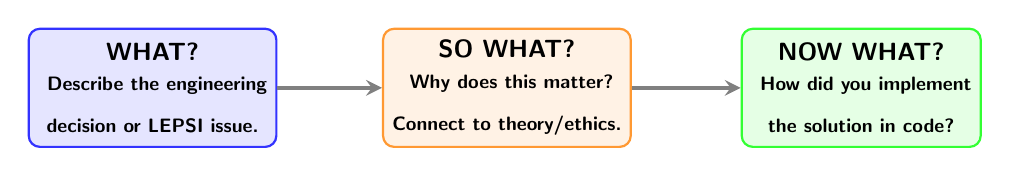
\begin{tikzpicture}[
        node distance=0.8cm and 1cm,
        box/.style={rectangle, draw=blue!80, fill=blue!10, thick, rounded corners, minimum width=3cm, minimum height=1.5cm, align=center, font=\small\bfseries},
        arrow/.style={->, >=stealth, line width=1.5pt, gray}
    ]
        % Nodes
        \node[box] (what) at (0,0) {WHAT?\\ \vspace{0.1cm} \scriptsize Describe the engineering\\ \scriptsize decision or LEPSI issue.};
        \node[box, fill=orange!10, draw=orange!80] (sowhat) at (4.5,0) {SO WHAT?\\ \vspace{0.1cm} \scriptsize Why does this matter?\\ \scriptsize Connect to theory/ethics.};
        \node[box, fill=green!10, draw=green!80] (nowwhat) at (9,0) {NOW WHAT?\\ \vspace{0.1cm} \scriptsize How did you implement\\ \scriptsize the solution in code?};
        
        % Arrows
        \draw[arrow] (what) -- (sowhat);
        \draw[arrow] (sowhat) -- (nowwhat);
    \end{tikzpicture}
    }
\end{frame}

\begin{frame}
    \frametitle{Example: Borton's Model in Action}
    \small
    \begin{itemize}
        \item \textbf{[WHAT]:} During development, I decided to implement strict Role-Based Access Control (RBAC) to restrict access to sensitive endpoints.
        \item \textbf{[SO WHAT]:} This addresses a critical LEPSI security concern. An autonomous system is a "dual-use" technology. If the system lacks authentication, it becomes vulnerable to hijacking, violating the ACM Code of Conduct regarding public safety.
        \item \textbf{[NOW WHAT]:} To solve this, I designed a middleware that decodes JWTs. If the payload lacks proper authorization, the system returns a 403 Forbidden status, ensuring hardware cannot be manipulated maliciously.
    \end{itemize}
\end{frame}

\begin{frame}
    \frametitle{Possible Reflection Themes}
    If you are structuring a reflection on a recent project, consider these themes:
    
    \begin{enumerate}
        \item \textbf{Security vs. Usability:} How did you balance making the system secure (RBAC, tokens) while adhering to WCAG accessibility guidelines?
        \item \textbf{Technical Debt:} What compromises did you make to hit a deadline, and how did you plan to refactor them?
        \item \textbf{Data Privacy:} How did you apply data minimisation principles to comply with GDPR?
        \item \textbf{Open Source Licensing:} What libraries did you use, and what are the legal implications if you commercialised the software?
    \end{enumerate}
\end{frame}

%------------------------------------------------------------
\section{Summary \& Conclusion}
%------------------------------------------------------------

\begin{frame}
    \frametitle{Module Wrap-Up}
    \small
    Over this module, you have transitioned from writing scripts to engineering software.
    
    \begin{itemize}
        \item You gathered requirements and designed architectures.
        \item You built full-stack applications.
        \item You isolated environments using Docker containerisation.
        \item You automated testing and delivery using CI/CD.
        \item You learned to clean your code and consider the ethical weight of what you build.
    \end{itemize}
    
    \vspace{0.3cm}
    \begin{center}
        \textbf{You are now equipped to operate as Professional Software Engineers.}
    \end{center}
\end{frame}

\begin{frame}
    \frametitle{Academic References \& Further Reading}
    \tiny
    \begin{itemize}
        \item \textbf{Decolonisation \& Data:} Couldry, N., \& Mejias, U. A. (2019). \textit{The Costs of Connection: How Data is Colonizing Human Life and Appropriating It for Capitalism}. Stanford University Press.
        \item \textbf{Palestine Surveillance Case:} Amnesty International (2023). \textit{Automated Apartheid: How Facial Recognition Fragments, Segregates and Controls Palestinians in the OPT}. \url{https://www.amnesty.org/en/latest/campaigns/2023/05/automated-apartheid/}
        \item \textbf{Occupation \& Control Framework:} Human Rights Watch (2021). \textit{A Threshold Crossed: Israeli Authorities and the Crimes of Apartheid and Persecution}. \url{https://www.hrw.org/report/2021/04/27/threshold-crossed/israeli-authorities-and-crimes-apartheid-and-persecution}
        \item \textbf{Digital Sovereignty \& Worldcoin:} Mutung'u, G., Martin, A., \& Brewczy\'nska, M. (2026). \textit{Regulatory entrepreneurship's threat to digital sovereignty: the case of Worldcoin in Kenya}. Science and Public Policy, 53(2), 289--299. \url{https://doi.org/10.1093/scipol/scag010}
        \item \textbf{AI Labour Extraction (Meta):} Perrigo, B. (2022). \textit{Inside Facebook's African Sweatshop}. TIME. \url{https://time.com/6147458/facebook-africa-content-moderation-employee-treatment/}
        \item \textbf{AI Labour Extraction (OpenAI):} Perrigo, B. (2023). \textit{OpenAI Used Kenyan Workers on Less Than \$2 Per Hour to Make ChatGPT Less Toxic}. TIME. \url{https://time.com/6247678/openai-chatgpt-kenya-workers/}
        \item \textbf{Algorithmic Bias:} Buolamwini, J., \& Gebru, T. (2018). \textit{Gender Shades: Intersectional Accuracy Disparities in Commercial Gender Classification}. Proceedings of Machine Learning Research.
        \item \textbf{Reflective Practice:} Borton, T. (1970). \textit{Reach, Touch, and Teach}. McGraw-Hill.
        \item \textbf{Professional Standards:} BCS / ACM Code of Ethics.
        \item \textbf{Information Security:} Merkow, M. S., \& Breithaupt, J. \textit{Information Security: Principles and Practices}.
    \end{itemize}
\end{frame}

\begin{frame}
    \frametitle{Q \& A}
    \begin{center}
        \Huge Any Questions?\\\vspace{0.5cm} 
        \normalsize fdelduchetto@lincoln.ac.uk
    \end{center}
\end{frame}

\end{document}